\section{Versuchsaufbau}
%skizze zum versuchsaufbau (oder foto) einf�gen,   es muss erkl�rt werden wie das ganze funktioniert und welche speziellen einstellungen verwendet wurden (z.b. welche kn�pfe an den ger�ten f�r die messung verdreht wurden)
Der Versuchsaufbau ist in Abbildung \ref{fig:aufbau} zu sehe. Die Hauptbestandteile sind die vier Szintillatoren (PM 1-4), welche jeweils noch mit einem Photomultiplier verbunden sind.

\begin{figure}[H]
	\centering
  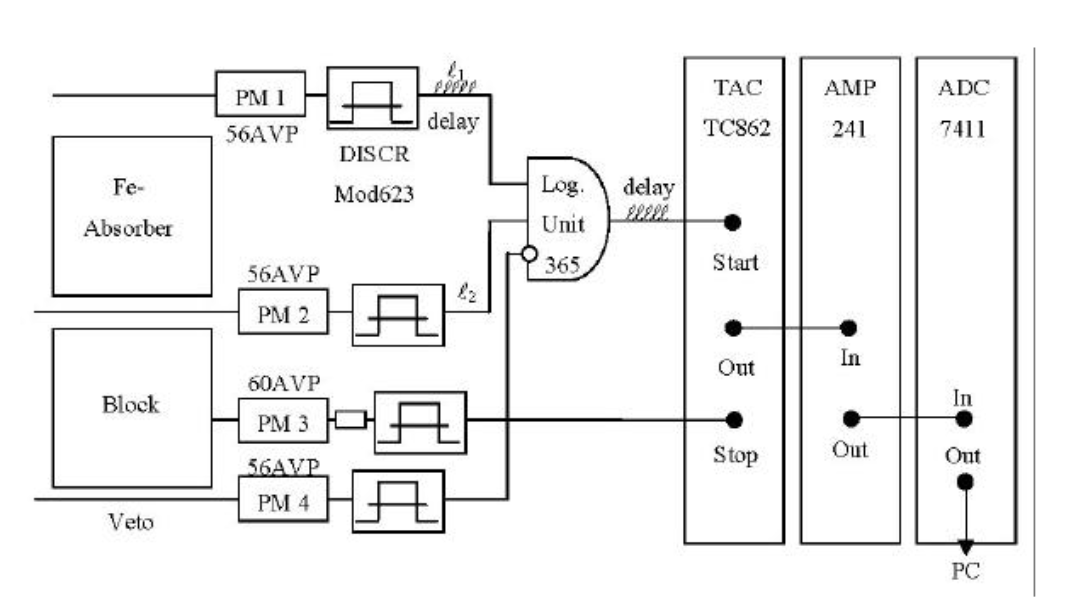
\includegraphics[scale=0.4]{unterdruekung.png}
	\caption{Schaltskizze des Versuchsaufbaus}
	\label{fig:aufbau}
\end{figure}

Der Szintillator f�r die Registrierung der Myonen ist PM3, es handelt sich um einen 25x25x25 cm$^3$ Plastikblock-Szintillator. PM1, PM2 und PM4 sind flach Szintillatoren, wobei PM4 als Veto fungiert, so dass nur Ereignisse die von PM3 noch registriert werden, jedoch nicht von PM4. PM1, PM2 und PM4 sind �ber eine logische Einheit an den Start-Pin des TAC angeschlossen. Der TAC wird gestartet, falls PM1 und PM2 ein Ereignis registrieren und PM4 keins registriert. Wenn PM4 auch noch das Myon registriert wird der TAC nicht gestartet, da das Myon nicht zerfallen ist. PM3 ist �ber den Photomuliplier an den Stop-Pin des TAC angeschlossen. Das Signal des TAC wird an einen Verst�rker (AMP) weiter geleitet, welche das Signal an einen Analog-Digital-Konverter (ADC) weitergibt. Es wurde noch ein Delay eingebaut, da die Szintillatoren ein unterschiedliches Baujahr haben (gr��ere Aufl�sungszeit) und die sich die Kabell�nge unterscheiden. Neben dem Universit�tsgeb�ude wir noch ein Eisenblock als Absorber verwendet, wodurch Myonen mit niedriger Energie vollst�ndig absorbiert werden und sich das Energiespektrum nach oben verschiebt. Der Vorteil des Absorbers ist, das andere Strahlung zum Teil vollst�ndig geblockt wird.

\subsection{Szintillationsz�hler}
Szintillationsz�hler werden zum detektieren von Strahlung verwendet. Des Szintialltionsz�hler besteht aus einem Szintillator, welcher gegen �u�eren Lichteinfall gesch�tzt ist und einem Photomulitplier zu verst�rken des Signals. Sie basieren darauf, dass der Szintillator durch die Strahlung ionisiert wird und Photonen abgibt, welche �ber einen Photomuliplier verst�rkt werden. Dadurch entsteht ein Strom an der Anode es Photmultipliers welchen meinstens �ber eine Digital-Analog-Konverter digitalisiert und an einen Computer weiter gegeben wird.

\subsection{Diskriminator}
Ein Diskriminator wandelt ein analoges Signal in ein digitales Signal mit einer Aufl�sung von einem Bit um. Es kann eine untere Schranke eingestellt werden, ab welcher eine 0 ausgegeben wird. Zus�tzlich kann auch eine obere Schranke eingestellt werde, sodass nur bei einer Spannung zwischen den Schranke eine 1 ausgegeben wird. Es ist auch einstellbar wie lange das Signal ausgegeben wird.

\subsection{Analog-Digital-Konverter}
Ein Analog-Digital-Konverter wandelt ein analoges Spannungssignal eine in digitales Spannungssignal um. Das Aufl�sungsverm�gen wird in Bit angegeben, je gr��er die Anzahl der Bits ist des so kleinschrittiger kann das analoge Signal aufgel�st werden. Die Umsetzungsgeschwindigkeit gibt an, wie lange es dauert eine �nderung des analogen Signals in ein digitales Signal umzuwandeln. 

\subsection{Delay}
Da verschiedene Signale nahezu zeitgleich ankommen m�ssen, werden einzelne Signale mit einem Delay versehe, damit sie zeitgleich ankommen. Das Delay wird meistens �ber l�ngere Kabel realisiert.

\subsection{Time-to-Amplitude-Converter(TAC)}
Ein TAC wird verwendet, um den Zeitlichen Abstand zwischen zwei Ereignissen zu bestimmen. Daf�r wird beim eintreffen eines Startsignals ein Kondensator linear aufgeladen, solange bis ein Stopsignal kommt und die Spannung an den Ausgang weitergegeben wird. Dadurch erh�lt man ein Spannungspuls der proportional zu der Zeitdifferenz zwischen Start- und Stopsignal ist. Als Besonderheit sei noch erw�hnt, dass der TAC im Jahr 1942 von Bruno Rossi zur Bestimmung der Lebensdauer von Myonen erfunden wurde.

\subsection{Multi-Channel-Analyser}
Mit einem Multi-Channel-Analyser werden Folgen von elektrischen Impulsen nach Gr��e geordnet und die Anzahl aufsummiert. Dies Daten k�nne als Histogramm dargestellt werden. Dabei wird jedem Kanal ein Energieintervall zugeordnet.

